\documentclass{article}
    % General document formatting
    \usepackage[margin=0.7in]{geometry}
    \usepackage[parfill]{parskip}
    \usepackage[utf8]{inputenc}
    
    % Related to math
    \usepackage{amsmath,amssymb,amsfonts,amsthm}
\usepackage{graphicx}
%\usepackage{subfig}
%\usepackage{subfigure}
\usepackage{caption}
\usepackage{subcaption}
\usepackage{listings}

\usepackage{titling}
%\usepackage{lipsum}

\usepackage{titlesec}

\titleformat*{\section}{\large\bfseries}
\titleformat*{\subsection}{\large\bfseries}
%\titleformat*{\subsubsection}{\large\bfseries}
%\titleformat*{\paragraph}{\large\bfseries}
%\titleformat*{\subparagraph}{\large\bfseries}
\titlespacing\section{0pt}{6pt plus 3pt minus 2pt}{0pt plus 2pt minus 2pt}
\titlespacing\subsection{0pt}{6pt plus 3pt minus 2pt}{0pt plus 2pt minus 2pt}
\titlespacing\subsubsection{0pt}{6pt plus 3pt minus 2pt}{0pt plus 2pt minus 2pt}

\pretitle{\begin{center}\large\bfseries}
\posttitle{\par\end{center}\vskip 0.01em}
\preauthor{\begin{center}\Large\ttfamily}
\postauthor{\end{center}}
\predate{\par\normalsize\centering}
\postdate{\par}

%\title{GI Assignment 3: A study of \textit{RB1} variation and regulation}
%\date{\today}

\begin{document}

%\maketitle

\begin{center}
\textbf{\Large{\centering{SP Assignment 3: Points, Points, and more Points}}}\\
\vspace{0.8mm}
\textbf{\textit{\small{USN: 303039534}}}
\end{center}
\vspace{1.3mm}


\section{Introduction}



\section{Results}

We start by implementing the Dmin model as described in the assignment and plot an example of a dmin simulation with parameters n=200, m=30, s=5 and ranges of x=[200:100] and y = [100:900]

\begin{figure}[h]
\centering
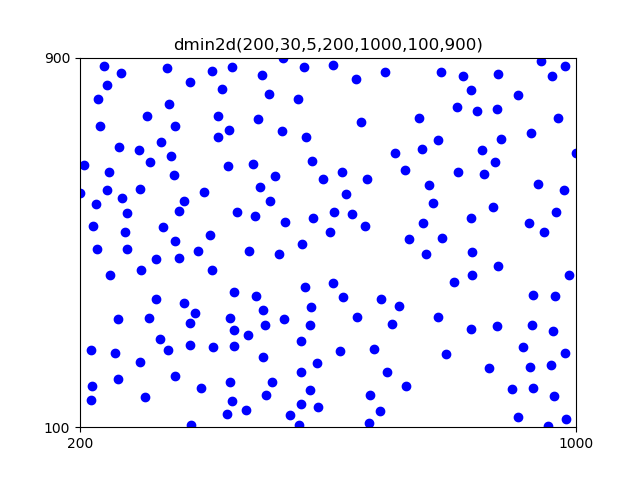
\includegraphics[width = 0.5\linewidth, trim={0 0 0 0}, clip=true]{dmin.png}
\caption{dmin model}
\label{fig:dmin}
\end{figure}

We proceed to implement a function calc\_RI to calculate the regularity index of a given pattern. The regularity index is defined as
\begin{equation}
	RI = \dfrac{\text{mean}(d_{ij}}{stdev(d_{ij})}
\end{equation} 
where $d_{ij}$ is the distance between points i and j.
This tells us how regular the spacing of points is; if all points have pairwise similar spacings, the standard deviation will be low and the regularity index high. If, on the other hand, pairwise distances differ a lot, the standard deviation will be high and the regularity index low. This is weighted by the mean distance to account for scalings of the grid.

We then generate 1000 dmin patterns with n=200, m=0, s=0, x=[0:1000], y=[0:1000]; i.e. we generate a square pattern of 200 points with no exclusion zone. We report the 50th largest value as a measure of regularity for this set of parameters. This is the boundary between the 5\% highest and 95\% lowest regularity indices we can achieve given this set of parameters, and thus tells us how regular a pattern we can expect to generate within a reasonable number of trials (here 20).

This gives a result of xxx. We can repeat this calculation 10 times which gives us a mean of xxx and an std of yyy indicating something.

We can investigate how this regularity index changes with both the number of points added and the shape of the grid. We constrain the area of the grid to 10\^6 giving us one degree of freedom specifying the shape, and we quantify this by the ratio of the two dimensions. We scan this ratio as well as the number of points added and report.

\begin{figure}[h]
\centering
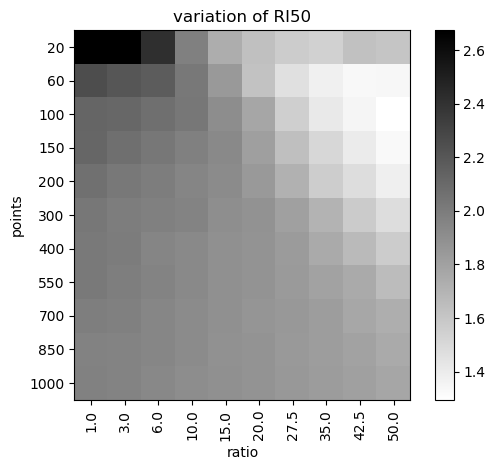
\includegraphics[width = 0.5\linewidth, trim={0 0 0 0}, clip=true]{RI50s_gray.png}
\caption{dependence of RI50 on n and ratio}
\label{fig:RI50}
\end{figure}

reproduce normal data. Start by scanning:

\begin{figure}[h]
\centering
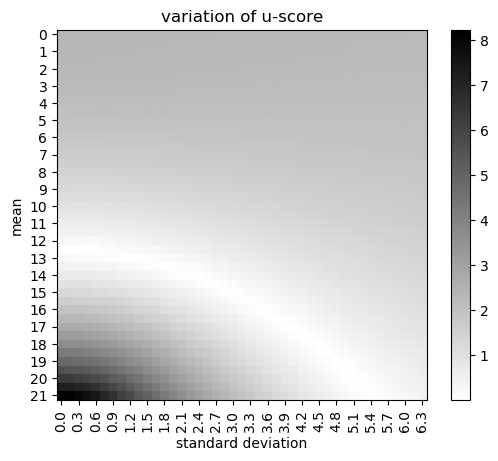
\includegraphics[width = 0.5\linewidth, trim={0 0 0 0}, clip=true]{similarity_gray_good.png}
\caption{similarity for different parameters}
\label{fig:sim}
\end{figure}

see that it's roughly 12 and 3; set niter=1000 - get sd = 0.11

Thus write steepest descent with threshold 0.2 (due to uncertainty in slope)

map line onto 3d plot

\begin{figure}[h]
\centering
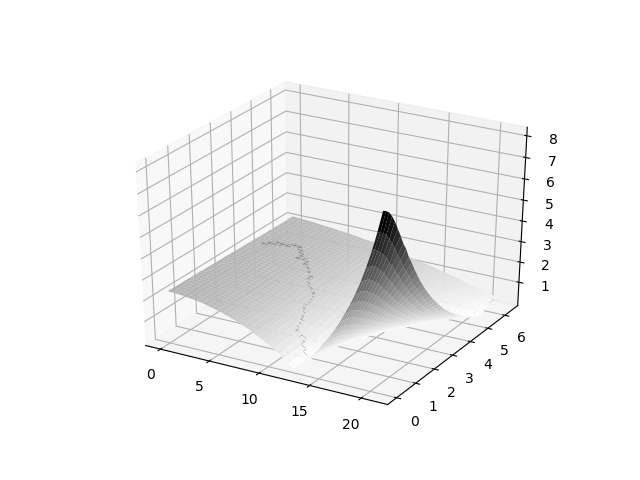
\includegraphics[width = 0.5\linewidth, trim={0 0 0 0}, clip=true]{project_descent.png}
\caption{similarity for different parameters}
\label{fig:sim}
\end{figure}

square packing:
21*21 = 441

separation: sqrt(20\^2-10\^2)
hexagonal: floor(400/sqrt(300)) = 23; i.e. 24 rows
12*(21+20) = 12*41 = 492


\begin{figure}[h]
	\centering
	\begin{subfigure}[t]{0.38\linewidth}
		\centering
		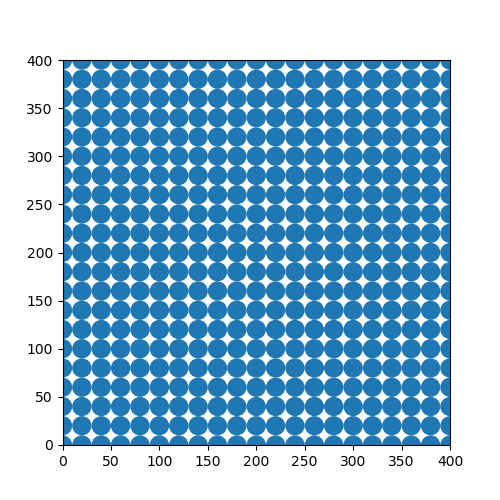
\includegraphics[width = 1.0\linewidth, trim={0 0 0 0}, clip=true]{square.png}
		\subcaption{}
		\label{fig:prot}	
	\end{subfigure}
	\hspace{0.06\linewidth}
	\begin{subfigure}[t]{0.38\linewidth}
		\centering
		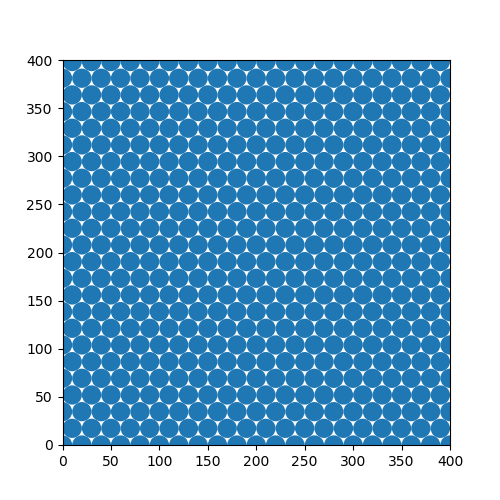
\includegraphics[width = 1.0\linewidth, trim={0 0 0 0}, clip=true]{hexagonal.png}
		\subcaption{}
		\label{fig:domains}	
	\end{subfigure}
\label{fig:4elj}
\caption{different packings.}
\end{figure}


\begin{figure}[h]
	\centering
	\begin{subfigure}[t]{0.38\linewidth}
		\centering
		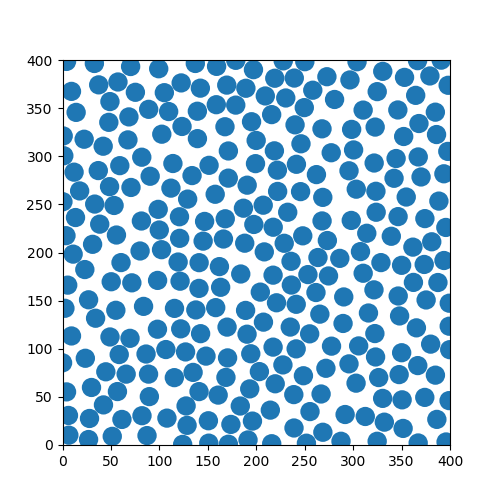
\includegraphics[width = 1.0\linewidth, trim={0 0 0 0}, clip=true]{plot_seq294.png}
		\subcaption{294 points generated by the sequential algorithm}
		\label{fig:prot}	
	\end{subfigure}
	\hspace{0.06\linewidth}
	\begin{subfigure}[t]{0.38\linewidth}
		\centering
		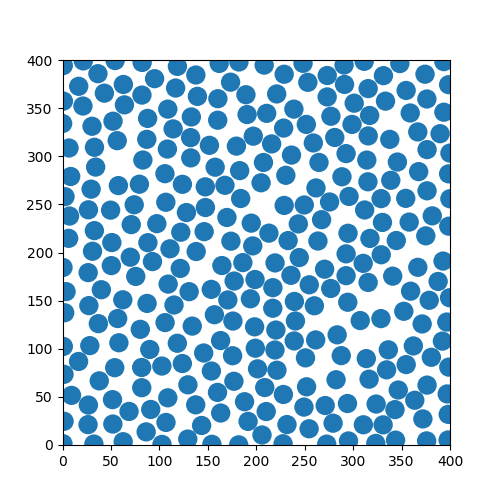
\includegraphics[width = 1.0\linewidth, trim={0 0 0 0}, clip=true]{plot_bd302.png}
		\subcaption{302 points generated by the epoch algorithm}
		\label{fig:domains}	
	\end{subfigure}
\label{fig:4elj}
\caption{different packings.}
\end{figure}



\begin{table}[h]
	\centering
	\begin{tabular}{ |c|c|c|c|c|c|c|c|c|c|c|c|c|c|}
		\hline
		\textit{H.sapiens} & S249 & T252 & T356 & T373 & S608 & S612 & S780 & S788 & S795 & S807 & S811 & T821 & T826 \\
		\hline
		\textit{C.jacchus} & S & T & T & T & S & S & S & S & S & S & S & T & T\\
		\textit{M.mulatta} & S & T & T & T & S & S & S & S & S & S & S & T & T\\
		\textit{F.catus} & S & T & T & T & S & S & S & S & S & S & \textbf{N} & T & T\\
		\textit{M.musculus} & S & T & T & T & S & S & S & S & S & S & S & T & T\\
		\textit{R.norvegicus}  & S & T & T & T & S & S & S & S & S & S & S & T & T\\
		\textit{G.gallus} & S & T & T & T & S & S & S & S & S & S & S & \textbf{S} & T\\
		\textit{M.gallopavo} & S & T & T & T & S & S & S & S & S & S & S & \textbf{S} & T\\
		\textit{I.punctatus} & S & T & T & T & S & \textbf{-} & S & S & S & S & S & \textbf{-} & T\\
		\textit{D.rerio} & S & T & T & T & S & \textbf{-} & S & S & S & S & S & \textbf{-} & T\\
		\hline
		RBL1 & F & L & T & Q & M & P & P & I & - & I & P & G & -\\
		RBL2 & - & N & K & P & R & P & P & V & A & I & Q & A & F\\
		\hline
	\end{tabular}
	\caption{Conservation of phosphorylation sites. Mismatches in orthologs have been highlighted in bold}
	\label{tab:align}
\end{table}



\section{Discussion \& Conclusion}



\section{Methods}



\section{References}
Chinnam \& Goodrich: "RB1, development, and cancer". \textit{Curr Top Dev Biol.} 94 (2013)\\
Dyson: "\textit{RB1}: "a prototype tumor supressor and an enigma", \textit{Genes and Development} 30 (2016)\\
Rubin: "Deciphering the Rb1 phosphorylation code", \textit{Trends Biochem Sci.} 38 (2013)\\
Narasimha et al.: "Cyclin D activates the Rb tumor suppressor by mono-phosphorylation", \textit{eLife} 3 (2014)\\
Turro et al.: "Haplotype and isoform specific expression estimation using multi-mapping RNA-seq reads", \textit{Genome Biology} 12 (2013)\\
Pearson \& Lipman: "Improved tools for biological sequence comparison", \textit{Proc Natl Acad Sci USA} 85 (1998)\\
Yam et al.: "Cyclin A in cell cycle control and cancer", \textit{Cell. Mol. Life Sci.} 59 (2002)

\section{Appendix (code)}

\lstset{basicstyle=\footnotesize}

%\large{File: parse\_pepvar.py}
%\lstinputlisting[language=python]{../code/parse_pepvar.py}


\end{document}

